\documentclass{article}
\usepackage[utf8]{inputenc}
\usepackage{amsmath}
\usepackage{amsfonts}
\usepackage{amsthm}
\usepackage{amssymb}
\usepackage{graphicx}
\usepackage{float}
\usepackage[margin=0.75in]{geometry}
\usepackage{xcolor}
\usepackage[makeroom]{cancel}
\usepackage{caption}
\usepackage{subcaption}
\usepackage{mwe}
\usepackage{hyperref}
% adds indent to first paragraph after section tag
\usepackage{indentfirst}
\theoremstyle{remark}
\newtheorem*{remark}{Remark}
% add tab command to file
\newcommand\tab[1][1cm]{\hspace*{#1}}
\newcommand{\R}{\mathbb{R}}
\newcommand{\N}{\mathbb{N}}
\newcommand{\norm}[1]{\left\lVert#1\right\rVert}
\renewcommand{\qedsymbol}{\rule{0.7em}{0.7em}}
\DeclareMathOperator{\Tr}{Tr}
\DeclareMathOperator{\spn}{span}
\title{Final Report: Reversible Architectures for Arbitrarily Deep Residual Neural Networks \\ \large Course 049064: Variational Methods in Image Processing}
\author{\small Jonathan Masin \& Netanel Rothschild}
\begin{document}
% remove date from title
\date{}
\maketitle
\section*{Background}
    Deep Residual Networks as of recently have been pushing state-of-the-art performance tasks with deeper and wider architectures. This paper 
has set out to interpret Deep Residual Networks as ordinary differential equations (ODEs). The motivation behind this, is the fact that 
ODEs have long been studied in mathematics and physics with rich theoretical and empirical success. Using this interpretation, the authors 
developed a theoretical framework on stability and reversibility of deep neural networks, the paper outlines three reversible neural network 
architectures that may go arbitrarily deep in theory. \par 
    The backbone of this paper is in proving the reversibility of the networks, which in turn allow for memory-efficient implementations, 
as they have no need to store the activation functions for most of the layers \par 
    The paper goes into detail of the theoretical background (which we will cover in this section) and demonstrates examples of experiments 
done, which we will replicate and improve on. Datasets used in the experiments are CIFAR-10, CIFAR-100, and STL-10. With baseline architectures 
used as comparisons. A major strength of the paper's implementation is that the models built using the theoretical background out perform 
strong baseline models, over fewer training data. \par 
    The authors claim the problem with Residual Networks is that, although widely used, there exist little theoretical analysis and guidelines for 
designing and training ResNets. This can be solved by viewing ResNets as ODEs as follows:
%2 images per row
\begin{figure}[H]
    \centering
    \begin{minipage}{0.45\textwidth}
        \centering
        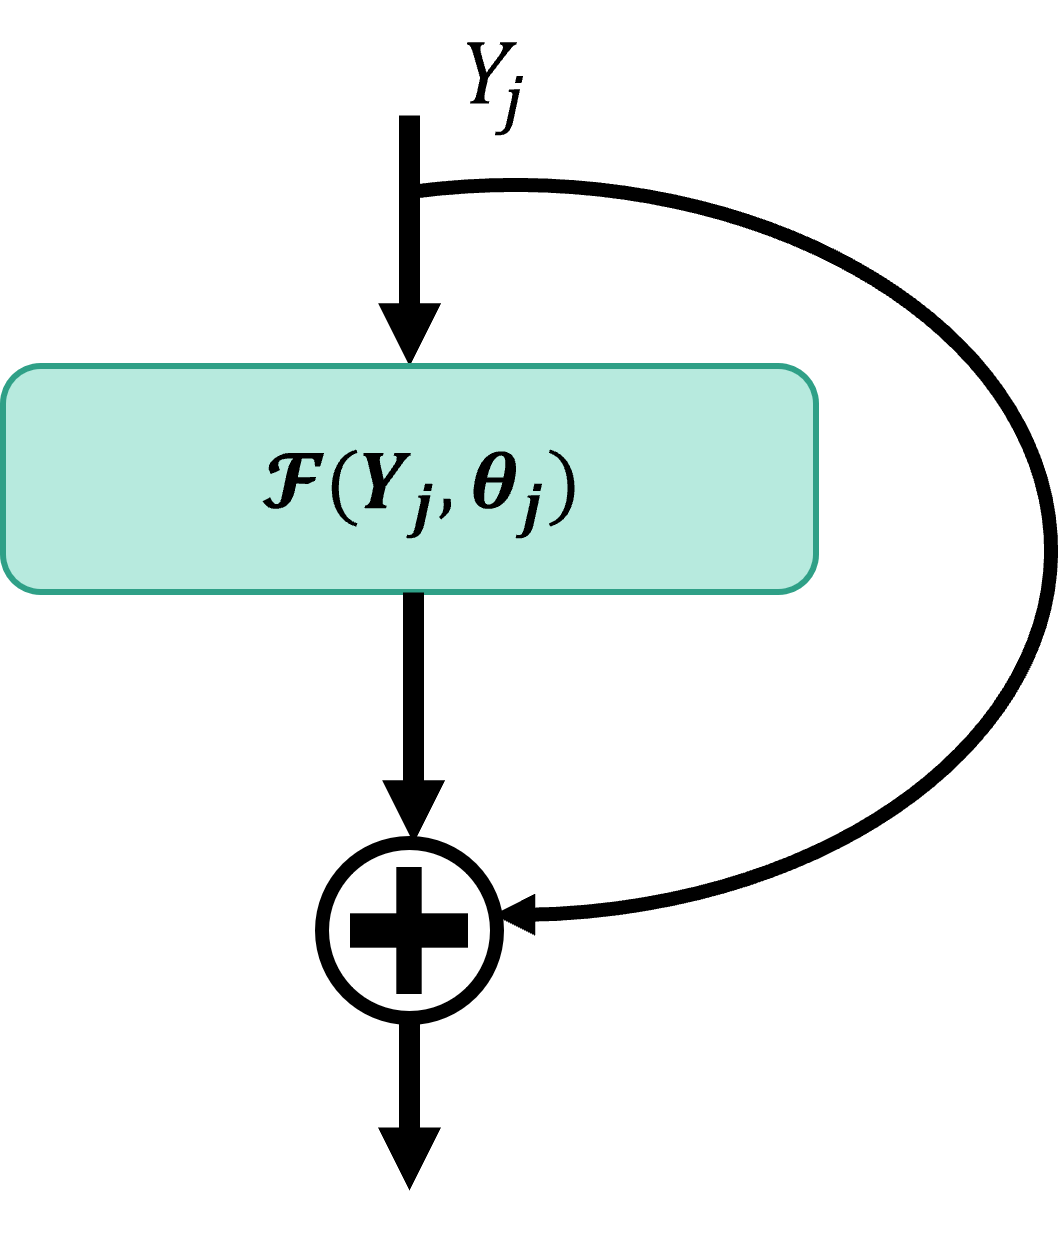
\includegraphics[scale=0.5]{imgs/residual_block.png} % first figure itself
        \caption{residual block}
    \end{minipage}\hfill
    \begin{minipage}{0.45\textwidth}
        \centering
        Output of block:
        \begin{gather}
            Y_{j+1} = Y_j + \mathcal{F}(Y_j, \theta_j) \nonumber \\
            \text{multiply by $h$} \nonumber  \\
            Y_{j+1} = Y_j + h\mathcal{F}(Y_j, \theta_j) \rightarrow \nonumber \\
            \mathcal{F}(Y_j, \theta_j) = \frac{Y_{j+1} - Y_j}{h} \nonumber \\
            \xrightarrow[]{h \rightarrow 0} \nonumber  \\
            \boxed{\dot{Y}(t) = \mathcal{F}(Y(t), \theta(t)); \ \ Y(0) = Y_0}
        \end{gather}
    \end{minipage}
\end{figure}

\par 
    A important definition to outline is "Reversibility", as it is the key element which allows for memory efficient implementations.\\
\textit{Definition Reversibility: An architecture is reversible if it allows the reconstruction of the activations going from the end to the beginning.}

\begin{figure}[H]
    \centering
    \begin{minipage}{0.45\textwidth}
        \centering
        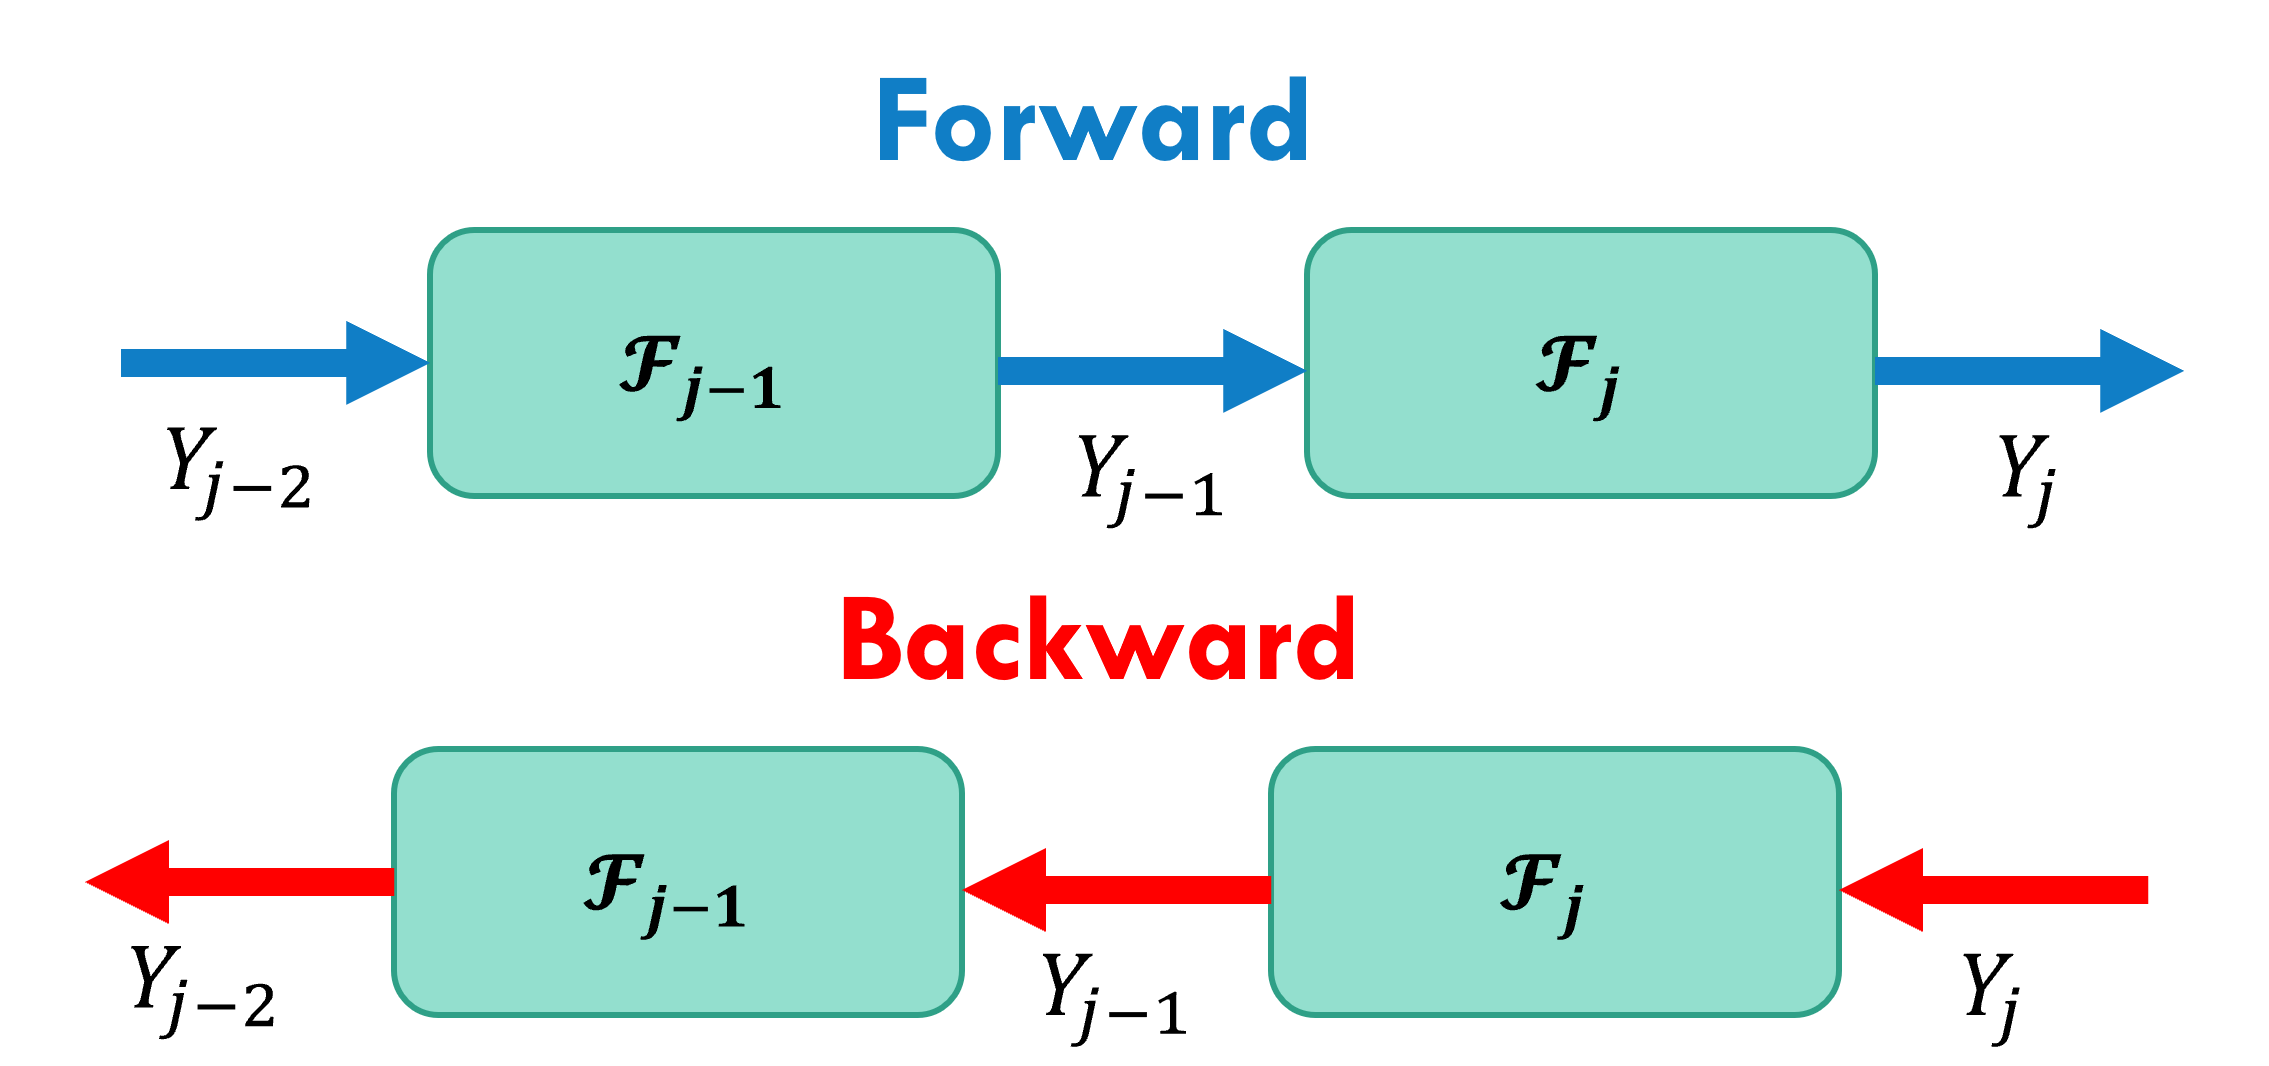
\includegraphics[scale=0.5]{imgs/revesibility_chart.png} % first figure itself
        \caption{forward and backward diagram}
    \end{minipage}\hfill
    \begin{minipage}{0.45\textwidth}
        \centering
        A network is reversible if for:
        \begin{gather*}
            Y_{j-2} = \mathcal{F}^{-1}_{j-1}(\mathcal{F}^{-1}_{j}(\dots \mathcal{F}^{-1}_{N}(Y_N)))\\
            Y_j = \mathcal{F}_{j}(\mathcal{F}_{j-1}(\dots \mathcal{F}_{N}(Y_0))) \\
            \mathcal{F}^{-1}_{k} \text{ Exists } \forall k \Rightarrow \text{Architecture is Reversible}
        \end{gather*}
    \end{minipage}
\end{figure}

Understanding how reversibility allows for a memory efficient implementations will be explored through an example further on, under the Section "Single Problem" \par

Another definition which is important to understand, which is derived from the realm of ODEs, stability. It is imortant to note that not every method that is algebraically reversible 
is numerically stable.\\

\textit{Definition Stability: A dynamical system is stable if a small change in the input data leads to a small change in the final result.} \\
\par 
To further better characterize this, assume a small perturbation, $\delta Y(0)$ to the initial data $Y(0)$, assume this change is propagated throughout the network. The question is, 
what would be the change after some time t, that is what is $\delta Y(t)$? This change can be characterized by the Lyapunov exponent $(\lambda)$:
\begin{gather*}
    \norm{\delta Y(t)} \approx e^{\lambda t} \norm{\delta Y(0)}
\end{gather*}
For a system, the "Forward Propagation" is well-posed (stable) when $\lambda \leq 0$, and ill-posed (unstable) if $\lambda > 0$. \\
It is easy to determine $\lambda$, as a bound on $\lambda$ can be derived from the eigenvalues of the Jacobian matrix of $\mathcal{F}$ with respect to $Y$, which is given by:
\begin{gather}
    J(t) = \nabla_{Y(t)} \mathcal{F}(Y(t)) \nonumber \\
    \text{A sufficient condition for stability is: } \nonumber \\
    \boxed{\max_{i = 1,2,\dots, n} Re(\lambda_i (J(t))) \leq 0, \ \ \forall t \in [0,T]} \\
    \text{where $\lambda_i(J)$ is the $i$th eigenvalue of $J$, and $Re(\cdot)$ denotes the real part} \nonumber
\end{gather}
Something the authors wanted to emphasis, the stability of the forward propagation is necessary to obtain stable networks that generalize well, but not sufficient. For a too small $\lambda$ 
the networks decay too quickly are not able to learn. This is why the authors suggest selecting networks with a negative $lambda \approx 0$

\section*{Previous Solutions}
    A paper titled "The reversible residual network: Backpropagation without storing activations" \cite{Gomez}, does similar work to this paper. Though the approach in the competing paper, set 
out to put limitations on the activation layer, that allow for the network to be reversible. Our paper in contrast, put no such limitations and instead chose to approach a solution the problem 
as layed out in the previous chapter through the use of ODEs. \par 
    Another famous paper which improves upon ResNet, is the famous ResNxt network. Published in the paper "Aggregated residual transformations for deep neural networks" \cite{ResNxt}. 
ResNxt introduces a homogeneous, multi-branch architecture to increase the accuracy. \par 
    Lastly worth mentioning is a paper titled "Deep networks with stochastic depth" \cite{stochastic depth}, which reduces the training time while increasing accuracy by randomly dropping a 
subset of layers and bypassing them with identity functions (similar to ResNet).

\pagebreak

\section*{Suggested Model}
    The authors present three different models in their paper:
    \begin{itemize}
        \item \textbf{Two-layer Hamiltonian Networks}
        \item \textbf{Midpoint Network}
        \item \textbf{Leapfrog Network}
    \end{itemize} \par 
    We will start by presenting the model we chose to present, implement and improve upon. This model's architecture is inspired by Hamiltonian systems
    \begin{gather*}
        \dot{Y}(t) = \sigma (K(t)Z(t) + b(t)) \\
        \dot{Z}(t) = -\sigma (K(t)^T Y(t) + b(t))
    \end{gather*}
    \par 
    $Y(t)$ and $Z(t)$ are partitions of the features, $\sigma$ is an activation function, and the network parameters are $\theta = (K,b)$. For convolutional neural networks $K(t)$ and $K^T(t)$ 
are convolutional operators. It can be shown that the Jacobian matrix of this ODE satisfies the condition of Ep.(2), leading to the conclusion that this network is stable and well-posed. 
The original Hamiltonian network \cite{Haber and Ruthotto} was designed using a single network. The authors claimed this was a limiting factor as the representability of a "single-layer" 
didn't generate satisfactory results. There for a "two-layer" architecture was suggested, which is what was used in the experimentation phase. The "two-layer" Hamiltonian equations are:
\begin{gather}
    \begin{split}
        \dot{Y}(t) = K^T_1(t) \sigma (K_1(t)Z(t) + b_1(t)) \\
        \dot{Z}(t) = -K^T_2(t) \sigma (K_2(t)Y(t) + b_2(t))
    \end{split}
\end{gather}

\begin{figure}[H]
    \centering
    \begin{minipage}{0.45\textwidth}
        \centering
        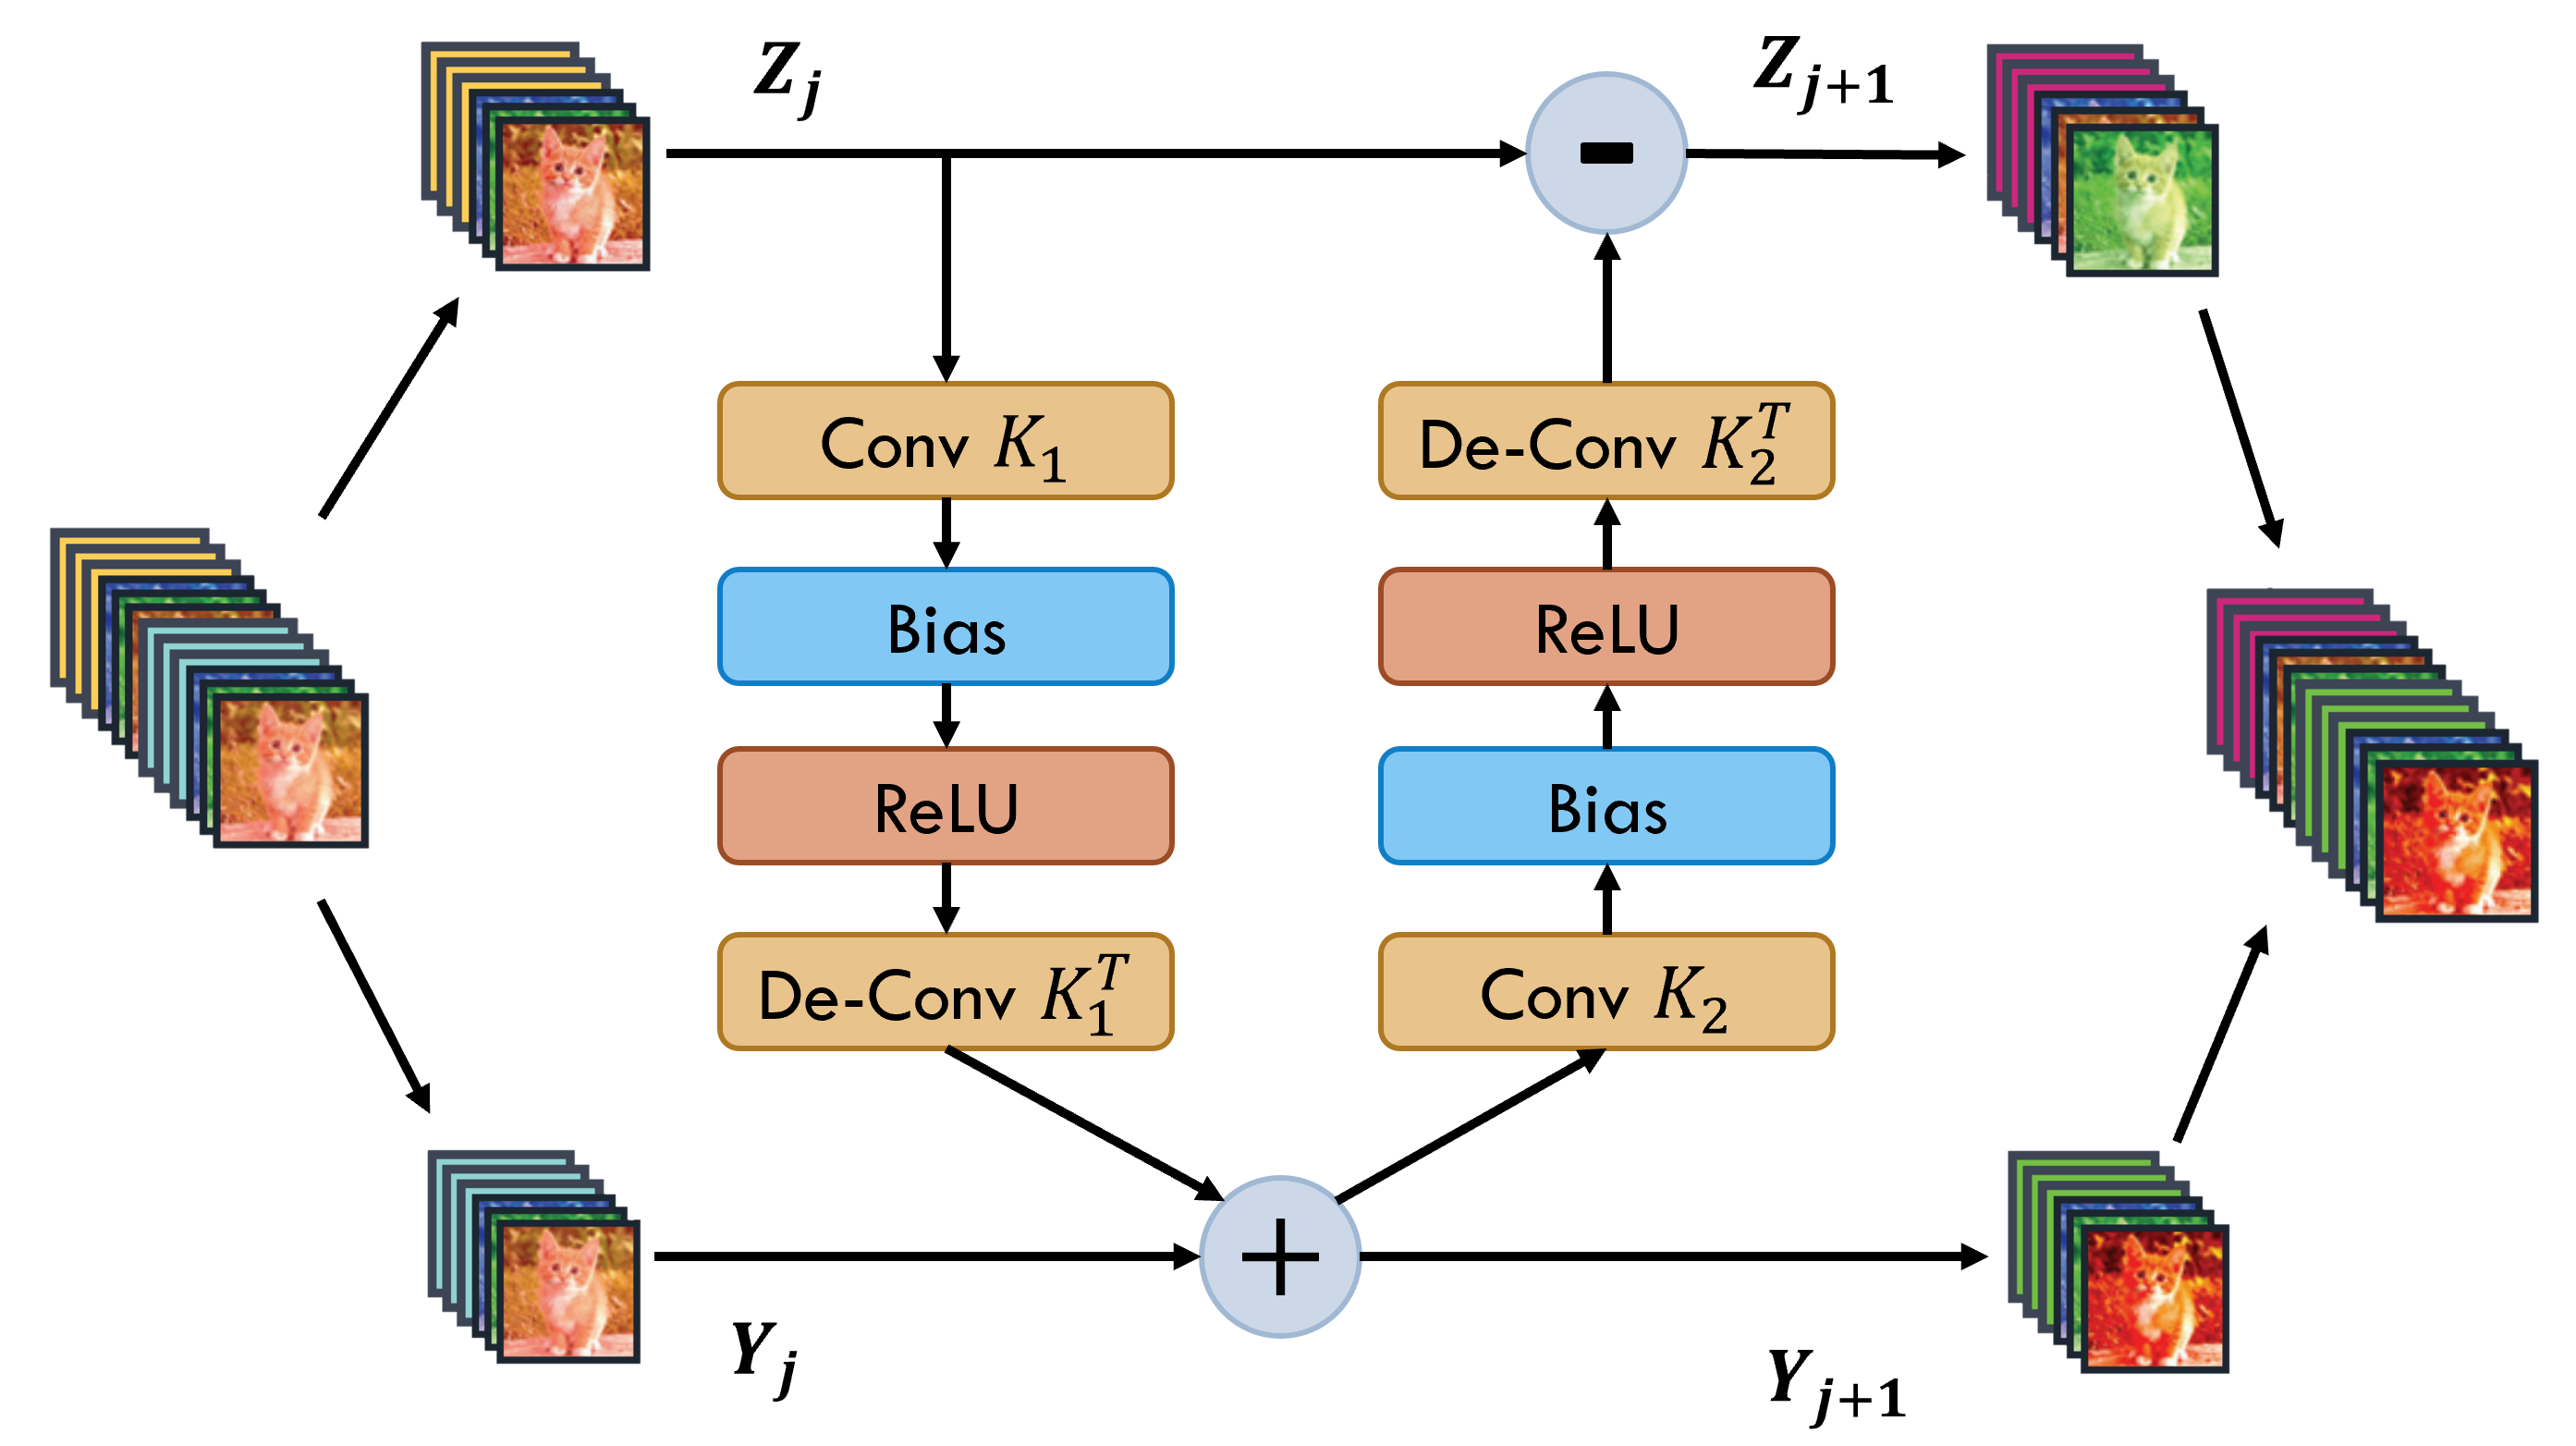
\includegraphics[width=\textwidth]{imgs/two_layer_hamiltonian_block.png} % first figure itself
        \caption{Two-Layer Hamiltonian}
    \end{minipage}\hfill
    \begin{minipage}{0.45\textwidth}
        \centering
        In discrete form (acquired using the Verlet method):
        \begin{gather*}
            Y_{j+1} = Y_{j} + h K^T_{j,1} \sigma (K_{j,1} Z_j + b_{j,1})) \\
            Z_{j+1} = Z_{j} - h K^T_{j,2} \sigma (K_{j,2} Y_{j+1} + b_{j,2}))
        \end{gather*}
    \end{minipage}
\end{figure}


\par 
    We will present a brief explanation of each of the other models. For the \textbf{Midpoint Network} the basis for it's model lays in the numerical 
method for discretization of the ODE as described in Eq.(1), done by using a central finite differences in time method: \\
\begin{gather*}
    \frac{Y_{j+1} - Y_{j-1}}{2h} = \mathcal{F}(Y_j) \\
    \text{Gives the following forward propagation } \\
    Y_{j+1} = Y_{j-1} + 2h \mathcal{F}(Y_j), \ \ \text{for } j = 1, \dots, N - 1
\end{gather*}
\par 
    The last model presented in the paper is the \textbf{Leapfrog Network}, which simply put is a special case of the Hamiltonian network Eq. (3), where one of the kernels is the identity 
matrix and one of the activations is the identity function. The leapfrog network involves two derivatives in time and reads 
\begin{gather*}
    \ddot{Y}(t) \approx h^{-2} (Y_{j+1} -2Y_j + Y_{j-1}) \\
    \xrightarrow[]{\text{Discrete Form}} \\
    Y_{j+1} = 
    \begin{cases}
        2Y_j - h^2 K^T_j \sigma (K_j Y_j + b_j),& j=1 \\
        2Y_j - Y_{j-1} - h^2 K^T_j \sigma (K_j Y_j + b_j),& j>0
    \end{cases}
\end{gather*}

Diagrams of Midpoint Network and Leapfrog Network blocks
%2 images per row
\begin{figure}[H]
    \centering
    \begin{minipage}{0.45\textwidth}
        \centering
        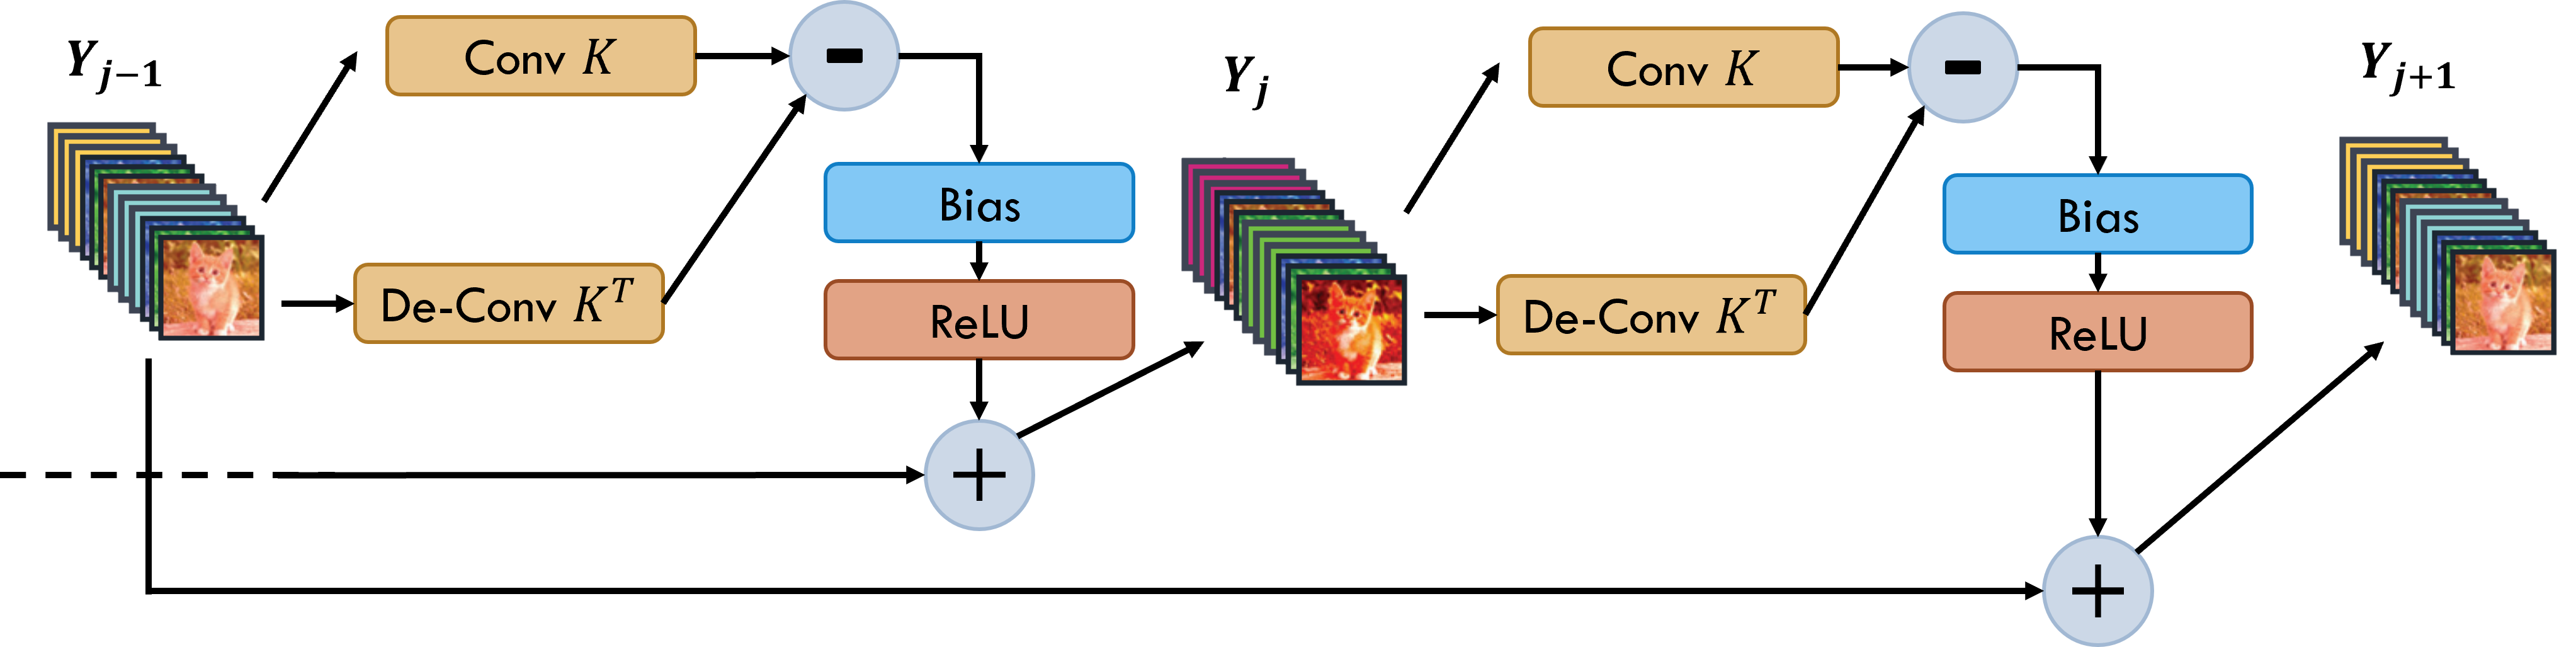
\includegraphics[width=\textwidth]{imgs/midpoint_block.png} % first figure itself
        \caption{Midpoint Network Block}
    \end{minipage}\hfill
    \begin{minipage}{0.45\textwidth}
        \centering
        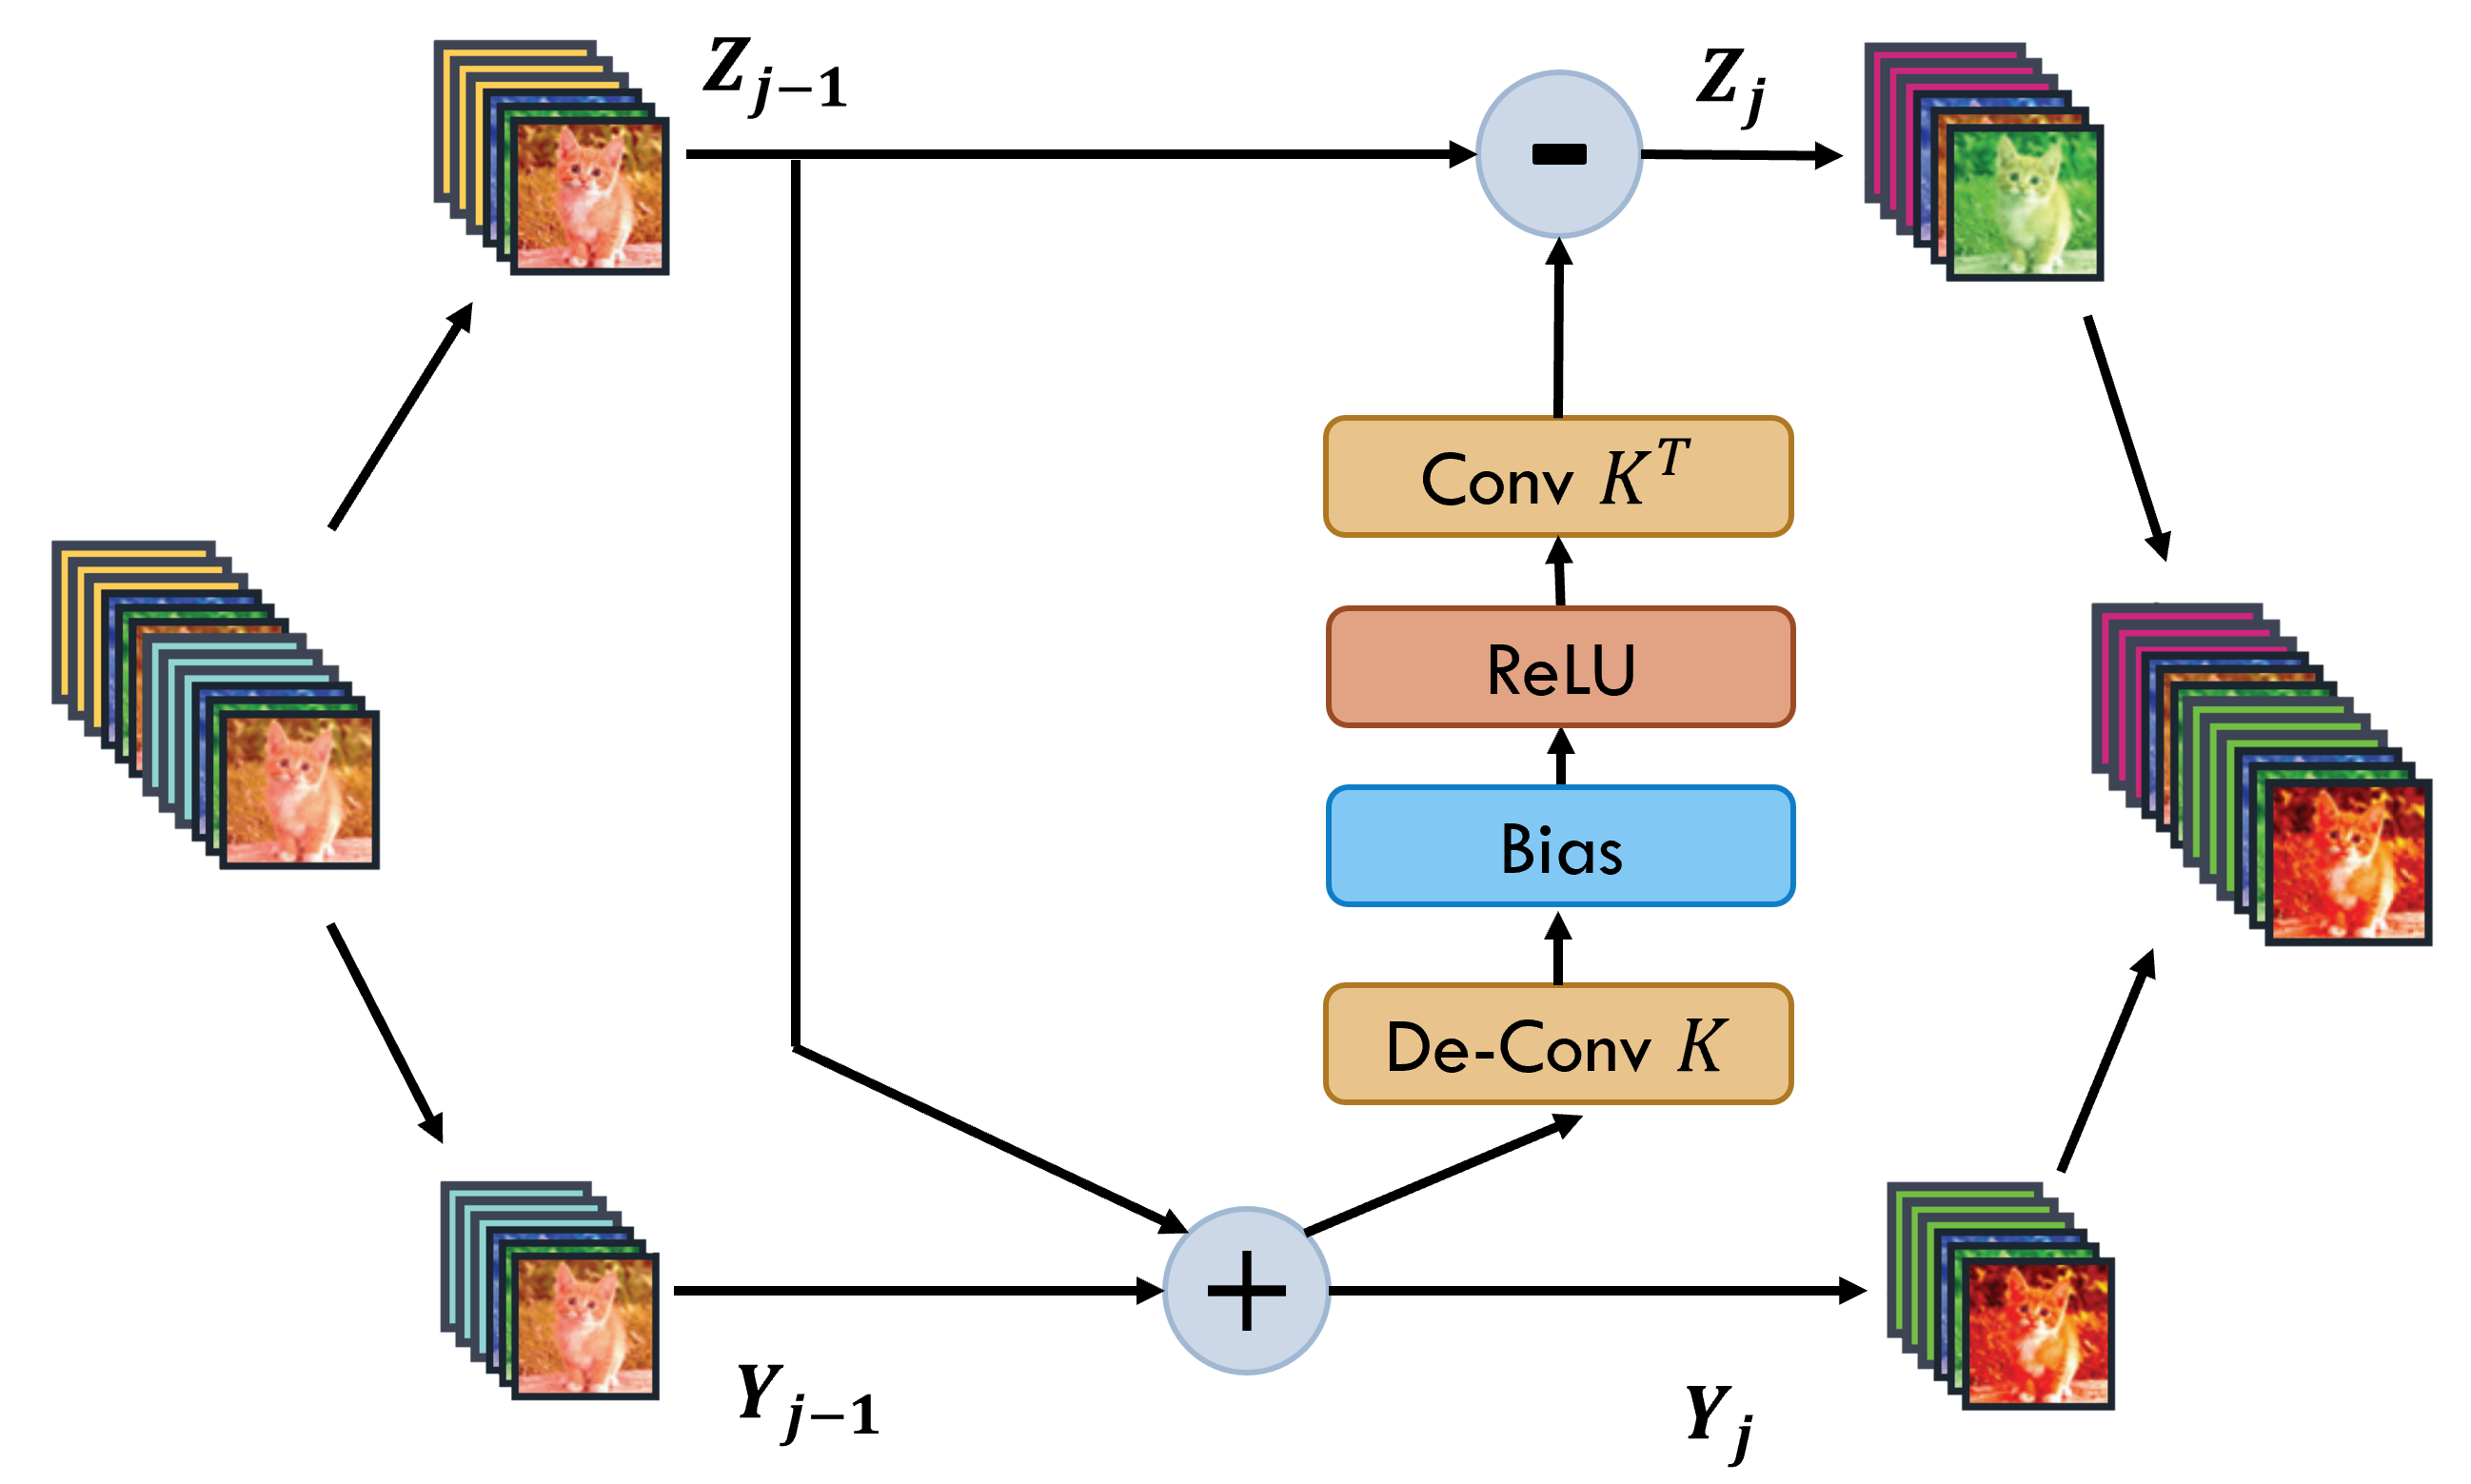
\includegraphics[width=\textwidth]{imgs/leap_frog_block.png} % second figure itself
        \caption{Leapfrog Network Block}
    \end{minipage}
\end{figure}
The blocks a chained together to make a neural network as depicted in the following diagram (Hamiltonian Network)

\begin{figure}[H]
    \centering
    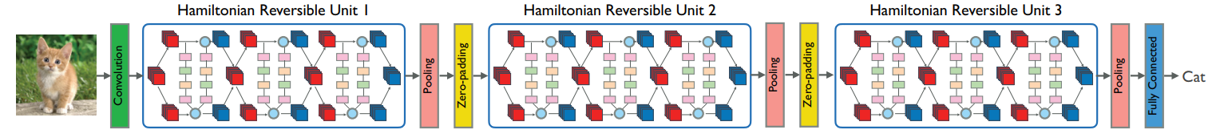
\includegraphics[width=\textwidth]{imgs/hamiltonian_network.png}    
\end{figure}

\section*{Implementation}
    We decided to implement the double layered Hamiltonian architecture. The writers of the paper implemented the model on MATLAB, without using the Deep Learning toolboxes that MATLAB 
provides. Our impression of the writer's implementation was that the code is hard to understand, and the code structure is confusing. In addition, their implementation relies on CudNN 
libraries that are not available for all. Due to all these factors we decided to implement the model with Python using the PyTorch library \cite{pytorch}. PyTorch is an open-source machine learning 
framework that builds deep neural networks on a tape-based automatic differentiation system (auto-grad). \par
    We will now go through the building stages of the model's framework, one module at a time, and understand each module's role in the model.\par
    First, we start by implementing the Residual Functions, i.e., the $\mathcal{F},\mathcal{G}$ blocks that are used in a reversible Hamiltonian block. The Residual Functions consist of a 
\textbf{convolutional layer} with a \textbf{bias term}, an \textbf{activation layer} (the paper suggested a Rectified Linear Unit, or ReLU) and a \textbf{transposed convolutional} layer 
with the \textit{same weights} as the convolutional layer (in the paper the convolutional weights are described by the matrix $K$). For the convolutional and transpose convolutional layers 
to share weights, we implemented the forward pass using Pytorch's functionals, inputting the same weight parameters for the convolution and transpose convolution functional.\par

The next module we implemented is the Reversible Hamiltonian Block, that is built using two Residual Functions ($\mathcal{F}$ block and $\mathcal{G}$ block) with the following architecture:
\begin{figure}[H]
    \centering
    \includegraphics[scale=0.5]{imgs/f_g_blocks.png}
\end{figure}
\par
To implement the minus sign at the end of the $\mathcal{G}$ block we added support in the Residual Function module with a field called 'sign' that takes values of $\{1,-1\}$ and multiplies 
the tensor by that value before outputting from the block. \par
Back to the Reversible Hamiltonian Block implementation, the input tensor is split along the channel dimension into two equal groups (as suggested by the paper) and each group moves 
through the block as described in the figure above. At the end of the block the two groups are concatenated back into one tensor, and it is moved to the next block. \par
The backward pass of the Reversible Hamiltonian Block incorporates the blocks reversibility, using the tensor from the following block to restore the activations of the current block. 
We carefully deleted any unused variables so now unused memory was stored, stressing the \underline{advantages of memory efficiency} of reversible architectures.\par
For the forward and backward passes of the Reversible Hamiltonian Block to be applied in the auto-grad framework, we implemented a \textbf{Reversible Unit Function} that wraps the forward and 
backward functions as static methods used by all reversible units.\par
Next, we implemented the Reversible Hamiltonian Unit, that is a sequence of several Reversible Hamiltonian Blocks chained together. The unit uses the Reversible Unit Function to apply 
forward and backward passes. \par
The Double layered Hamiltonian Network is comprised out of 3 Reversible Hamiltonian units, with average pooling between each layer. In addition, a convolution layer is added before the 
first unit and a fully connected layer is added to the output of the final unit. After each Reversible Hamiltonian Unit, the number of channels is doubled using zero padding. \par
In addition, we implemented the \textbf{weight smoothness decay regularization} in the PyTorch framework. This type of regularization is not supported by the default PyTorch optimizers and 
losses, therefore we were required to write a custom regularization function that computed the weight smoothness regularization term. The weight smoothness is calculated by penalizing the 
difference between the current weights and the weights before the optimizer step $\Sigma \norm{W_j - W_{j-1}}^2_F$. We defined a weight cache to store the weights from the previous state 
(before the optimization step). \par
For training we used the hyper-parameters suggested by the paper: initial learning rate of $0.01$, batch size of $128$, momentum of $0.9$, weight decay of $2\cdot 10^{-4}$ and weight 
smoothness decay of $2\cdot 10^{-4}$. The learning rate was decreased by a factor of $10$ in epochs $80, 120, 160$. We trained on $200$ epochs with validation steps every $20$ epochs. 
We split the training data 10\% for validation and the rest for training.\par
We performed our experiments using the CIFAR10\cite{cifar10} dataset on the Hamiltonian-218 network (18 Hamiltonian blocks per unit). We trained using a NVIDIA GeForce 2080 GPU that 
accelerated our training. Training time (when using the GPU) was approximately 27 seconds per epoch.

\pagebreak

\section*{Analysis}
    Let us examine some of the results displayed in the paper. When examining the experimental results two main points jump out:
\begin{enumerate}
    \item The accuracry of the suggested models perform poorly compared with the baseline models (on the CIF datasets)
    \item The suggested models require significantly fewer parameters to train (as promised by the authors) and in turn perform better than the 
    baseline models, on a subset of training data.
\end{enumerate}

\begin{figure}[H]
    \centering
    \includegraphics[scale=0.5]{imgs/cifar_results.png}
    \caption{Poor performance (\textcolor{red}{Red}), On par performance (\textcolor{yellow}{Yellow}), Superior performance (\textcolor{green}{Green}). Fewer Parameters (\textcolor{violet}{Violet})}
\end{figure}
\begin{figure}[H]
    \centering
    \includegraphics[scale=0.5]{imgs/substrata_data.png}
    \caption{Both on CIFAR and STL datasets we set how the Hamiltonian network outperforms for "small" datasets (subset is \% complete dataset)}
\end{figure}

We selected the Hamiltonian Network as the model to further investigate, as it seemed to be the most mentioned in the paper. With it being the most experimented on, and most data about it 
available. So gauging our implementation would have ample data to compare with.


\pagebreak
\section*{Creative and Suggested Improvements}
    As noted in the Analysis section, there is much left to be desired with regard to accuracy of the models offered by the paper. We have decided to address this issue with two approaches. 
The first approach is adding batch normalization and dropout layers to tackle over-fitting we experienced during training the original model. The second improvement was adding "inception 
blocks" (first introduced in "Going deeper with Convolutions"\cite{C. Szegedy}) to $\mathcal{F}$ and $\mathcal{G}$ blocks. \par
First we will explain the justification behind inception blocks. \par
When designing a convolutional network, it is often difficult to select the best kernel size. Inception blocks seek to overcome this by incorporating several kernels of various sizes and 
applying them all at each stage. This has proven to be effective. The models tend to go "wider" (authors terminology) and require more computations, but improve the accuracy of the network. 
For us to be able to include these inception blocks in a Two-Layer Hamiltonian network for example, we must first prove that neither of the assumptions the Hamiltonian network guarantees, 
are violated. We will prove both "reversibility" and "stability" still apply to our model. \\
\begin{figure}[H]
    \centering
    \includegraphics[scale=0.5]{imgs/inception_block.png}
\end{figure}
Two-Layer Hamiltonian-Inception Block:

\begin{gather*}
    Y_{j+1} = Y_{j} + h K^T_{j,1} \sigma (K_{j,1} Z_j + b_{j,1})) \\
    Z_{j+1} = Z_{j} - h K^T_{j,2} \sigma (K_{j,2} Y_{j+1} + b_{j,2}))
\end{gather*}
    
Here we will present the proof that the inception block can be represented as a kernel K. This would in turn show the model with inception blocks to be: 1) Stable, 2) Reversible \\
We use the following block in our model: \\
\begin{figure}[H]
    \centering
    \includegraphics[scale=0.5]{imgs/our_inception_block.png}
\end{figure}
$1 \times 1$, $3 \times 3$, $5 \times 5$ are convolution operators with kernel sizes $1, 3, 5$ and the filter concatenation is an element wise summation of the output channels.\\
Notice here we implemented a variation of the inception block, which includes a skip connection (a linear operator).\\
\begin{proof}\ \\
\textit{Convolutional operators are linear}\cite{Signals and Systems}\\
\begin{gather*}
    \forall A,B \text{ linear operators } \rightarrow AB = C \text{ is also a linear operator }\\
\end{gather*}
\textit{we know that a sum of linear operators are also a linear operator}\\
\begin{gather*}
    \Rightarrow I(x) = C_{1 \times 1} x + C_{3 \times 3} C_{1 \times 1} x + C_{5 \times 5} C_{1 \times 1} x = (C_{1 \times 1} + C_{3 \times 3} C_{1 \times 1} + C_{5 \times 5} C_{1 \times 1}) x \\
    \Rightarrow I(x) = Kx
\end{gather*}
\end{proof} \par
Back to our implementation. \par
For our first approach, we added batch normalization after the initial convolution layer and a dropout layer with factor 0.4 before the fully connected layer. These two regularization 
methods help tackle \textit{overfitting} that we encountered during the training of the original architecture. Both methods are well known and are commonly used in deep neural networks. 
From our analysis they do not harm the reversibility and stability of the Hamiltonian blocks (as they are outside of the blocks) thus they promise to improve the results. \par
Batch normalization re-centers and re-scales each batch, smoothing the objective function and helping the optimization to find the global minima. Dropout layers are activated only during 
training. They “de-activate” neurons with a probability of a Bernoulli distribution with a factor p (in our case p=0.4). Dropout encourages the network to learn a sparse representation as 
a side-effect.\\
We trained the Regularized Hamiltonian Network in the same manner as the original network, with a difference of using $5\cdot 10^{-4}$ weight decay. \par

The second improvement we added was adding inception to the $\mathcal{F}$ and $\mathcal{G}$ blocks. We did this by splitting the $\mathcal{F}$ or $\mathcal{G}$ block input into 4 groups. 
One was passed as a skip connection. The second was passed through a 1x1 convolution layer. The third was passed through a 1x1 and then 3x3 convolution layers and the last group was 
passed through 1x1 and then 5x5 convolution layers. Afterwards, the 4 groups were concatenated and continued to an activation layer (ReLU). Finally, the tensor was split again into 4 and 
the same process was done only with transpose convolution layers with shared weights to the initial convolution layers. At the end of the block the groups were concatenated, and the 
tensor continued its flow. The architecture is described in the following figure:
\begin{figure}[H]
    \centering
    \includegraphics[scale=0.5]{imgs/f_g_inception.png}
\end{figure} \par
We trained the Inception Hamiltonian network on 250 epochs, with initial learning rate of 0.001 and weight decay of $5\cdot 10^{-4}$. All the other hyper-parameters were the same as in 
the training of the original network. The training time for the Inception Hamiltonian network (while using a GPU) was approximately 48 seconds per epoch. \\

Presented here is a table with our final scores:

\begin{center}
    \begin{tabular}{||c c c||} 
        \hline
        Model & Train Loss & Test Acc \\ [0.5ex] 
        \hline\hline
        Original Network & 2.05 & 96\% \\ 
        \hline
        Original Network + batch normalization \& dropout & 1.62 & 97\% \\
        \hline
        Inception block Network & 1.08 & 68\% \\ 
        \hline
    \end{tabular}
\end{center}
First thing to stand out, is the low Test accuracy for our inception implementation. We spent many hours trying to asses and improve this, but our code is correct and the accuracy is 
accurate which leaves us with the conclusion, inception blocks \underline{don't always improve the model}. While this was disappointing to discover, we want to note, we still were able to 
improve on the original authors models. Our network with dropout and batch-normalization, out performed the original model.\\
Progress of each model through the Training phase:
\begin{figure}[H]
    \centering
    \includegraphics[width=0.45\textwidth]{imgs/original_acc.jpeg}
    \caption{Accuracy - Original Model}
\end{figure}
%2 images per row
\begin{figure}[H]
    \centering
    \begin{minipage}{0.45\textwidth}
        \centering
        \includegraphics[width=\textwidth]{imgs/dropout_acc.jpg} % first figure itself
        \caption{Accuracy - Model with dropout and batch-normalization added}
    \end{minipage}\hfill
    \begin{minipage}{0.45\textwidth}
        \centering
        \includegraphics[width=\textwidth]{imgs/dropout_loss.jpeg} % second figure itself
        \caption{Loss - Model with dropout and batch-normalization added}
    \end{minipage}
\end{figure}
\begin{figure}[H]
    \centering
    \begin{minipage}{0.45\textwidth}
        \centering
        \includegraphics[width=\textwidth]{imgs/inception_acc.jpeg} % first figure itself
        \caption{Accuracy - Model with dropout and batch-normalization added}
    \end{minipage}\hfill
    \begin{minipage}{0.45\textwidth}
        \centering
        \includegraphics[width=\textwidth]{imgs/inception_loss.jpeg} % second figure itself
        \caption{Loss - Model with dropout and batch-normalization added}
    \end{minipage}
\end{figure}

Lastly a very important table which may offer a clue as to why the Inception Block performed so poorly.\\

\begin{center}
    \begin{tabular}{||c c c c||} 
        \hline
        \ & Original Network & Original Network + batch normalization \& dropout & Inception block Network\\ [0.5ex] 
        \hline\hline
        Number of params & 1,751,882 & 1,751,946 & 458,682 \\
        \hline
    \end{tabular}
\end{center}

We can see a significant decrease in the number of parameters in the Inception block network, with the same amount of layers. Our conclusion is that perhaps the model did not have enough 
parameters to reach significant enough model.

\pagebreak
\section*{Conclusion}
We started this project with an idea in mind, we were unsure if it would succeed but talked at length about the different approaches we could take, and selected the one we felt was most 
promising. A lot of what we learned throughout the project was novel to us and required learning beyond the scope of the course. Implementation of the paper was no small task, our full 
repository can be found here: \href{https://github.com/nateRot/049064_variational_methods_in_image_processing/tree/main/final_project}{Github}. \par
As mentioned early on we had a short correspondence with the authors of the paper, seeking their implementation. But their repository seemed lacking and not up to date. It was missing 
models and the code was not entirely consistent with the paper. \par
Researching DNN can be a bit tricky and in many cases it comes down to experimental data, attempting certain changes and noting a performance increase or decrease. While here in the final 
report we noted the improvements, they were not achieved immediately, and our model went through many unsuccessful iterations. \par 
We feel satisfied with our final result, as it reached the goal of improving upon the original authors solution and did not degrade in any way the performance. Though it should be noted 
our original research question (can we improve the models by incorporating inception blocks?) did not meet expectations, while remaining within the frame of the paper.\par
Some future possibilities to further expand on, at the very basic level, develop improved models for the other models suggested by the authors (Leapfrog Network, Midpoint Network). Perhaps 
expand on some of our original ideas exploring other networks not suggested by the paper, using PDE's, including finding models with a higher order PDE. Though after a lengthy discussion 
we concluded most models suggested based on higher order PDE's would require numeric solutions which in turn would be difficult to prove stability as defined in the paper. \\
Lastly at the time of writing this summary we are running some final tests on a much larger inception network (the authors who published the inception blocked, recommended it only be used 
on very large networks. Though no details on what large meant.), with hopes that an increase in layers would in turn increase the number of parameters, but we would be comparing a more 
complex network with the original 218 layer one. Therefore comparison would not be an equal evaluation.

\pagebreak
\begin{thebibliography}{9}

    \bibitem{Gomez}
        Gomez, A. N.; Ren, M.; Urtasun, R.; and Grosse, R. B. 2017.
        The reversible residual network: Backpropagation without storing
        activations. NIPS.

    \bibitem{ResNxt}
        Xie, S.; Girshick, R.; Doll, P.; Tu, Z.; and He, K. 2017. 
        Aggregated residual transformations for deep neural networks. CVPR.

    \bibitem{stochastic depth}
        Huang, G.; Sun, Y.; Liu, Z.; Sedra, D.; and Weinberger, K. Q. 2016.
        Deep networks with stochastic depth. In ECCV.

    \bibitem{Haber and Ruthotto}
        Haber, E., and Ruthotto, L. 2017. Stable architectures for deep
        neural networks. arXiv preprint arXiv:1705.03341

    \bibitem{pytorch}
    Adam Paszke, Sam Gross, Francisco Massa, Adam Lerer, James Bradbury, Gregory Chanan, Trevor Killeen, Zeming Lin, Natalia Gimelshein, Luca Antiga, Alban Desmaison, Andreas Kopf, 
    Edward Yang, Zachary DeVito, Martin Raison, Alykhan Tejani, Sasank Chilamkurthy, Benoit Steiner, Lu Fang, Junjie Bai, and Soumith Chintala. 
    Pytorch: An imperative style, high-performance deep learning library. In NeurIPS, 2019.

    \bibitem{cifar10}
    https://www.cs.toronto.edu/~kriz/cifar.html
    
    \bibitem{C. Szegedy}
    C. Szegedy, W Liu, Y. Jia, P. Sermanet, S. Reed, D. Anguelov, D. Erhan, 
    V. Vanhoucke, A. Rabinovich. 2017.
    Going deeper with convolutions. arXiv preprint arXiv:1409.4842v1

    \bibitem{Signals and Systems}
    Hayes, Signals and Systems, p. 11.


\end{thebibliography}

\end{document}


